\documentclass[tikz,border=5pt]{standalone}
\usepackage[utf8]{inputenc}
\usepackage[T1]{fontenc}
\usepackage{lmodern,amsmath,amssymb}
\usepackage[american]{circuitikz}
\usepackage{pgfplots}
\pgfplotsset{compat=1.18}
\usetikzlibrary{circuits.logic.US,positioning,calc,arrows.meta,patterns,shapes.geometric}
\definecolor{Primary}{HTML}{1F77B4}
\begin{document}
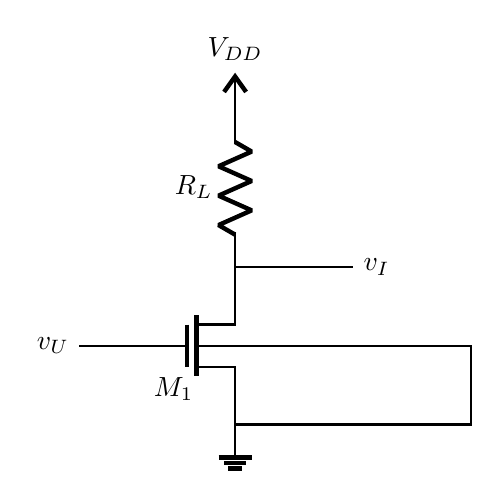
\begin{tikzpicture}[thick]\node[nmos,bulk](m1)at(0,0){};\draw(m1.G)--++(-1,0)node[left]{$v_U$};\draw(m1.S)--(0,-1)node[ground]{};\draw(m1.bulk)--(3,0)--(3,-1)--(0,-1);\draw(m1.D)--(0,1)--(1.5,1)node[right]{$v_I$};\node[left]at(-.4,-.55){$M_1$};\draw(0,1)to[R,l=$R_L$](0,3)node[vcc]{$V_{DD}$};\end{tikzpicture}
\end{document}
